Gomoku, also known as Five-in-a-row, originated from Japan and is very popular around the world. Two players put Go pieces (black and white stones) strategically on square size board, usually 15x15 or 19x19. The objective for any player is to have 5 pieces in a row. Figure~\ref{fig:board} is an example of what a Gomoku board may look like. Due to the two player zero-sum nature of the game, we can effectively leverage a game tree search algorithm like the minimax algorithm.\\
\\
For clarity sake, we will elaborate on what a game tree is and what it represents. In essence, a game tree is a directed graph where in which the nodes represent different board states and the edges represents move that a player can take from that given board state. Figure~\ref{fig:gametree} is an example of a game tree. The root node represents the initial board state and all its children are the potential next board state and so on and so forth. We use tic-tac-toe as an example here but the structure and idea is the same regardless of the game. The term depth is used for game trees in the same way as with graphs -  the distance between the leaf and root nodes. Hence, the game tree of Figure~\ref{fig:gametree} is of depth=2.\\
\\
In discussing Gomoku's game tree search, we will also touch on the complexity of we are trying to accomplish. The term \textit{complexity} in the context of games denote two different measures, \textit{state-space complexity} and \textit{game-tree complexity}. State-space complexity refers to the number of legal game positions reachable from the initial positions of the game. This contrasts with game-tree complexity which is defined as the number of leaf nodes in the solution search tree from the initial board state. \cite{allis_1994} As Allis writes, the game-tree complexity is what determines the size of minimax search tree needed to completely solve the game. Allis also includes Figure~\ref{fig:complexity} that shows the relative estimated game complexities. Notice that Gomoku, third from the right, is among the most complex games with a game-tree complexity of around $10^{80}$. In comparison, games like Othello with $10^{30}$ possible leaf nodes and chess with $10^{60}$ possible leaf nodes are relatively less complex. However, Go, the game from which Gomoku originates, is known to be the one of the most complex games with $10^{170}$ leaf nodes. It should be noted here that Allis estimates Gomoku's complexity with a 15x15 board and this will drastically change with a different sized board.\\

\begin{figure}[ht]
    \centering
    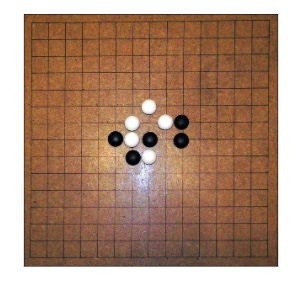
\includegraphics[scale=0.5]{images/gomoku_board.png}
    \caption{An example gomoku board}
    \label{fig:board}
\end{figure}

\begin{figure}[ht]
    \centering
    
\includegraphics[scale=0.40]{images/gametree.png}
    \caption{An example game tree}
    \label{fig:gametree}
\end{figure}


\begin{figure}[ht]
    \centering
    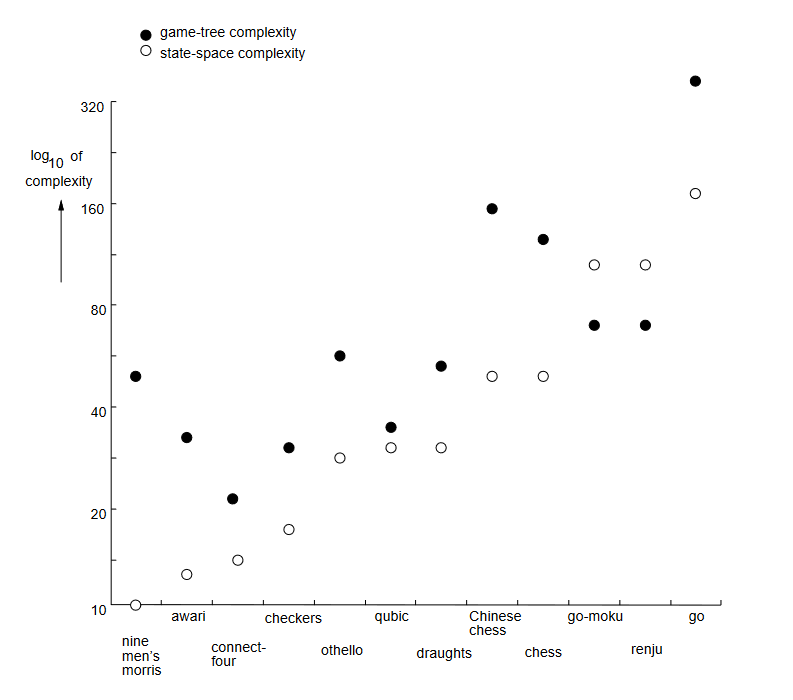
\includegraphics[scale=0.58]{images/complexity.PNG}
    \caption{Estimated game complexities \cite{allis_1994}}
    \label{fig:complexity}
\end{figure}

\noindent
Now, if there were a technology that could search through all $10^{80}$ leaf nodes, then we would be able to exactly calculate the best next move. However, exhaustively searching through all leaf nodes to determine the best move is infeasible and unrealistic. Therefore, we limit the size of the game tree by its depth. That is, we search the game tree up to some depth $d$ and determine the best move from that smaller game tree. Naturally, there is a trade-off between, $d$ and the how 'good' our best move is and this is an especially important consideration because our game tree increases exponentially in size as we increase the search depth. A larger tree would give us more information to determine the best move, but at the same time, would take much longer. One way to reduce the number of leaf nodes that we have to explore is through branch pruning and this can be done via alpha-beta pruning. (To be explained in Section~\ref{sec:minimax}). However, branch pruning alone proves to be insufficient if we are to search at a larger depth. The motivation of a parallel implementation is to improve on the computation time so that we are able to increase our search space without sacrificing accuracy. With this work, we present parallel implementations of Gomoku's game tree search using OpenMP, CUDA and other optimizations that we implemented.\\
